%! Author = silva
%! Date = 6/6/2022


\chapter{Introduction}\label{ch:intro}



The images were obtained to better understand Parkinson's disease.


\section{Datasets}\label{sec:dataset}

We have two datasets of microscopy images which both consist of several ten thousands.
Once we have "cell_type_1" and "cell_type_2".


\captionsetup{labelformat=empty}
\begin{figure}[ht!]
    \begin{minipage}[t]{\linewidth}
        \centering
        \begin{minipage}[t]{0.49\linewidth}
            
\includegraphics[width=\textwidth, keepaspectratio]{./graphics/dataset_sample_1.png}  %  <<< image name 1
        \end{minipage}
        \begin{minipage}[t]{0.49\linewidth}
            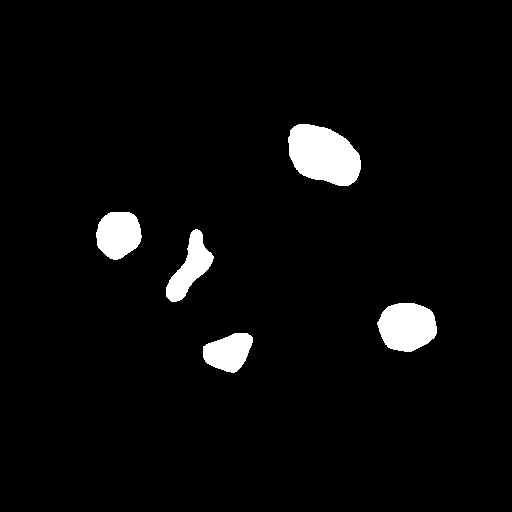
\includegraphics[width=\textwidth, keepaspectratio]{./graphics/dataset_sample_1_label.png}  %  <<< image name 1
        \end{minipage}
    \end{minipage}

    \begin{minipage}[t]{\linewidth}
        \begin{minipage}[t]{0.49\linewidth}
            
\includegraphics[width=\textwidth, keepaspectratio]{./graphics/dataset_sample_2.png}  %  <<< image name 1
        \end{minipage}
        \begin{minipage}[t]{0.49\linewidth}
            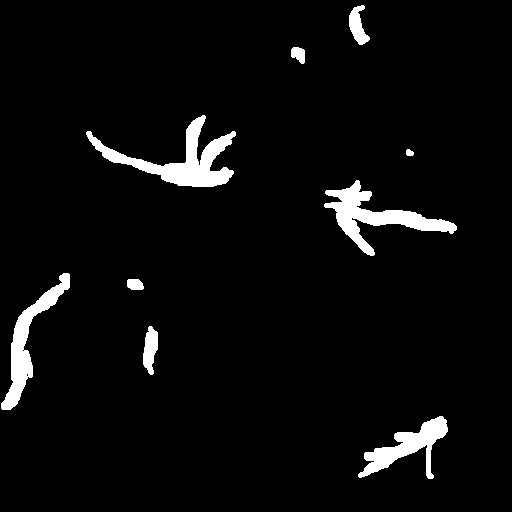
\includegraphics[width=\textwidth, keepaspectratio]{./graphics/dataset_sample_2_label.png}  %  <<< image name 1
        \end{minipage}
    \end{minipage}
    \label{fig:1}
    \caption{Dataset 2: Datasets }
\end{figure}


\section{haha2}

